\documentclass{article}

\usepackage{fancyhdr}
\usepackage{extramarks}
\usepackage{amsmath}
\usepackage{amsthm}
\usepackage{amsfonts}
\usepackage{tikz}
\usepackage[plain]{algorithm}
\usepackage{algpseudocode}
\usepackage{enumerate}
\usepackage{amssymb}

\usetikzlibrary{automata,positioning}

%
% Basic Document Settings
%

\topmargin=-0.45in
\evensidemargin=0in
\oddsidemargin=0in
\textwidth=6.5in
\textheight=9.0in
\headsep=0.25in

\linespread{1.1}

\pagestyle{fancy}
\lhead{\hmwkAuthorName}
\chead{\hmwkClass\ (\hmwkClassInstructor\ \hmwkClassTime): \hmwkTitle}
\rhead{\firstxmark}
\lfoot{\lastxmark}
\cfoot{\thepage}

\renewcommand\headrulewidth{0.4pt}
\renewcommand\footrulewidth{0.4pt}

\setlength\parindent{0pt}

%
% Create Problem Sections
%

\newcommand{\enterProblemHeader}[1]{
    \nobreak\extramarks{}{Problem \arabic{#1} continued on next page\ldots}\nobreak{}
    \nobreak\extramarks{Problem \arabic{#1} (continued)}{Problem \arabic{#1} continued on next page\ldots}\nobreak{}
}

\newcommand{\exitProblemHeader}[1]{
    \nobreak\extramarks{Problem \arabic{#1} (continued)}{Problem \arabic{#1} continued on next page\ldots}\nobreak{}
    \stepcounter{#1}
    \nobreak\extramarks{Problem \arabic{#1}}{}\nobreak{}
}

\setcounter{secnumdepth}{0}
\newcounter{partCounter}
\newcounter{homeworkProblemCounter}
\setcounter{homeworkProblemCounter}{1}
\nobreak\extramarks{Problem \arabic{homeworkProblemCounter}}{}\nobreak{}

%
% Homework Problem Environment
%
% This environment takes an optional argument. When given, it will adjust the
% problem counter. This is useful for when the problems given for your
% assignment aren't sequential. See the last 3 problems of this template for an
% example.
%
\newenvironment{homeworkProblem}[1][-1]{
    \ifnum#1>0
        \setcounter{homeworkProblemCounter}{#1}
    \fi
    \section{Problem \arabic{homeworkProblemCounter}}
    \setcounter{partCounter}{1}
    \enterProblemHeader{homeworkProblemCounter}
}{
    \exitProblemHeader{homeworkProblemCounter}
}

%
% Homework Details
%   - Title
%   - Due date
%   - Class
%   - Section/Time
%   - Instructor
%   - Author
%

\newcommand{\hmwkTitle}{Tutorial 6}
\newcommand{\hmwkDueDate}{February 23, 2021}
\newcommand{\hmwkClass}{CZ2003}
\newcommand{\hmwkClassTime}{SS3}
\newcommand{\hmwkClassInstructor}{Assoc Prof Alexei Sourin}
\newcommand{\hmwkAuthorName}{\textbf{Pang Yu Shao}}
\newcommand{\hmwkAuthorID}{\textbf{U1721680D}}

%
% Title Page
%

\title{
    \vspace{2in}
    \textmd{\textbf{\hmwkClass:\ \hmwkTitle}}\\
    \normalsize\vspace{0.1in}\small{Due\ on\ \hmwkDueDate\ at 10:30am}\\
    \vspace{0.1in}\large{\textit{\hmwkClassInstructor\ - \hmwkClassTime}}
    \vspace{3in}\\
    \hmwkAuthorName\\
    \hmwkAuthorID
}

\date{22/02/2021}

\renewcommand{\part}[1]{\textbf{\large Part \Alph{partCounter}}\stepcounter{partCounter}\\}

%
% Various Helper Commands
%

% Useful for algorithms
\newcommand{\alg}[1]{\textsc{\bfseries \footnotesize #1}}

% For derivatives
\newcommand{\deriv}[1]{\frac{\mathrm{d}}{\mathrm{d}x} (#1)}

% For partial derivatives
\newcommand{\pderiv}[2]{\frac{\partial}{\partial #1} (#2)}

% Integral dx
\newcommand{\dx}{\mathrm{d}x}

% Alias for the Solution section header
\newcommand{\solution}{\textbf{\large Solution}}

% Probability commands: Expectation, Variance, Covariance, Bias
\newcommand{\E}{\mathrm{E}}
\newcommand{\Var}{\mathrm{Var}}
\newcommand{\Cov}{\mathrm{Cov}}
\newcommand{\Bias}{\mathrm{Bias}}

\begin{document}

\maketitle

\pagebreak

\begin{homeworkProblem}
    Define the three-dimensional solid object displayed in Figure Q1
    \begin{enumerate}
        \item by functions \(x(u,v,w)\), \(y(u,v,w)\), \(z(u,v,w)\), \(u\in [0,1]\), \(v\in [0,1]\)
        \item by functions \(f(x,y,z) \geq 0\) 
    \end{enumerate}
    \begin{figure}[H]
        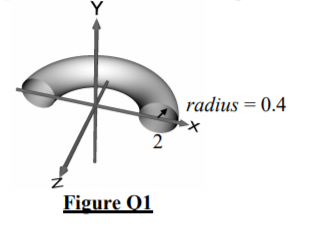
\includegraphics[width=6cm]{fig/q1.PNG}
        \centering
    \end{figure}
    

    \textbf{Solution}\\
    Part 1:\\
    Draw 2D surface,\\
    Using bilinear representation:
    \(P = P1 + u(P2 - P1) + v(P3 - P1 + u(P4 - P3 – (P2 - P1)))\)\\
    \(P1 = (-3, 1, 0)\), \(P2 = (3, 1, 0)\),  \(P3 = (-3, 3, 0)\),  \(P4 = (0, 3, 0)\), \\\\

    \(x(u,v) = -3 + u(3-(-3)) + v(-3 - (-3) + u(0 - (-3) – (3 - (-3))))\)\\
    \(x(u,v) = -3 + 6u - 3vu\)\\

    \(y(u,v) = 1 + u(1 - 1) + v(3 - 1 + u(3 - 3 - (1 - 1)))\)\\
    \(y(u,v) = 1 + 2v\)\\\\
    To get solid, sweep z with third parameter from -0.5 to 1:\\
    \(x(u,v,w) = -3 + 6u - 3vu\)\\
    \(y(u,v,w) = 1 + 2v\)\\
    \(z(u,v,w) = -0.5 + 1.5w\)\\
    \(u,v,w \in [0,1]\)
    \begin{figure}[H]
        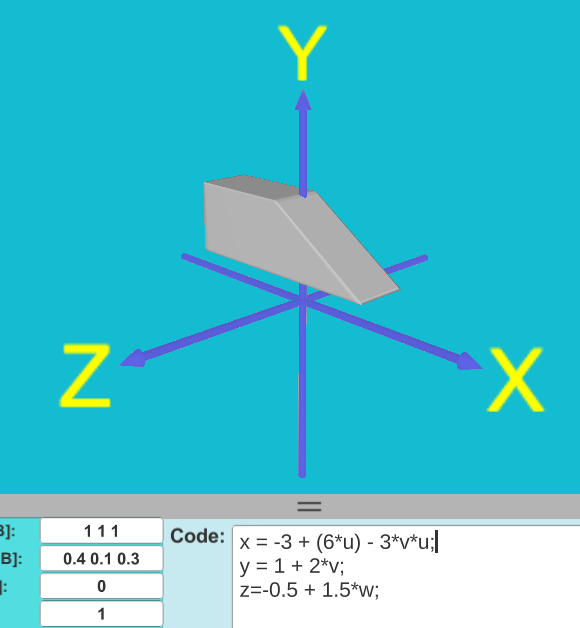
\includegraphics[width=6cm]{fig/q1a.PNG}
        \centering
    \end{figure}

    Part 2:\\
    Components to form solid:
    \begin{enumerate}
        \item \(x \geq -3\), or \(x + 3 \geq 0\)
        \item \(x \leq 3\), or \(3 - x \geq 0\)
        \item \(y \geq 1\), or \(y - 1 \geq 0\)
        \item \(y \leq 3\), or \(3 - y \geq 0\)
        \item \(\frac{x}{-3/(-2/3)} + \frac{y}{3} - 1 \geq 0\), or \(2x + 3y - 9 \geq 0\)
        \item \(z \geq -0.5\), or \(z + 0.5 \geq 0\)
        \item \(z \leq 1\), or \(1 - z \geq 0\)
    \end{enumerate}
    \(\therefore f(x,y,z): min(x+3, 3-x, 3-y, 2x +3y - 9, z + 0.5, 1-z) \geq 0\)
    \begin{figure}[H]
        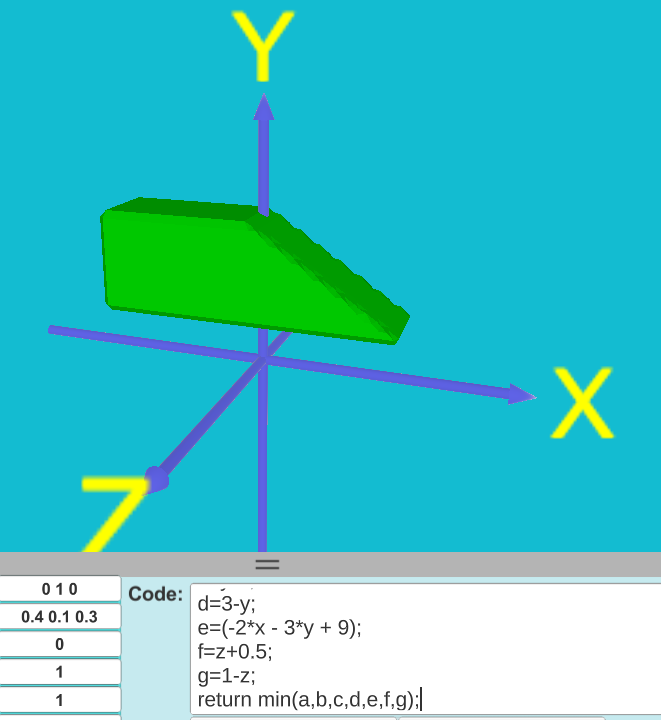
\includegraphics[width=6cm]{fig/q1b.PNG}
        \centering
    \end{figure}
    

    

\end{homeworkProblem}
\pagebreak
\begin{homeworkProblem}
    A curve displayed in Figure Q2 (left) is defined in polar coordinates r and a by
    the function \(r = 1.2 sin(2\alpha - 0.5\pi)\), \(\alpha \in [0,2\pi]\). Propose parametric
    functions \(x(u, v)\), \(y (u, v)\), \(u, v \in [0, 1]\) defining the 2D solid shape located in
    the XY Cartesian coordinates system as it is displayed in Figure Q2 (right).
    \begin{figure}[H]
        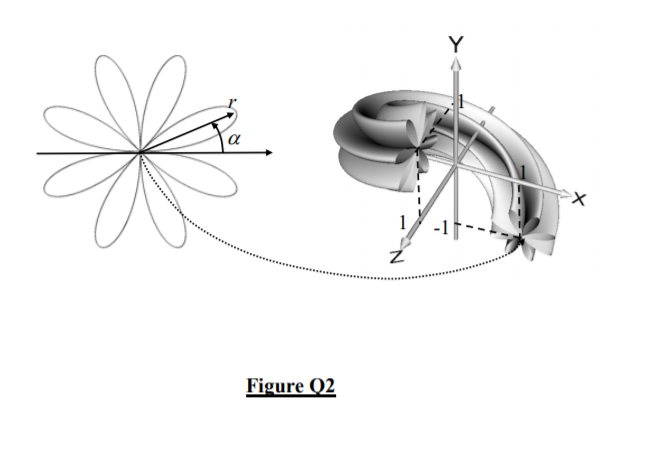
\includegraphics[width=10cm]{fig/q2.PNG}
        \centering
    \end{figure}

    \textbf{Solution}\\
    \(r = 1.2sin(2\alpha-0.5\pi)\)\\\\
    \(x(u) = rcos(2\pi u)\)\\
    \(y(u) = rsin(2\pi u)\)\\\\

    \(x(u) = 1.2sin(4\pi u-0.5\pi)cos(2\pi u)\)\\
    \(y(u) = 1.2sin(4\pi u-0.5\pi)sin(2\pi u)\)\\\\
    Offset by (1.2,1.2):\\
    \(x(u) = 1.2+1.2sin(4\pi u-0.5\pi)cos(2\pi u)\)\\
    \(y(u) = 1.2+1.2sin(4\pi u-0.5\pi)sin(2\pi u)\)\\
    Radius changes from (0.5 to 1.2), incorporate this information using parameter \textbf{v}:\\
    \(x(u,v) = 1.2+(0.5 + 0.7*v)sin(4\pi u-0.5\pi)cos(2\pi u)\)\\
    \(y(u,v) = 1.2+(0.5 + 0.7*v)sin(4\pi u-0.5\pi)sin(2\pi u)\)\\
    \(u,v \in [0,1]\)
    \begin{figure}[H]
        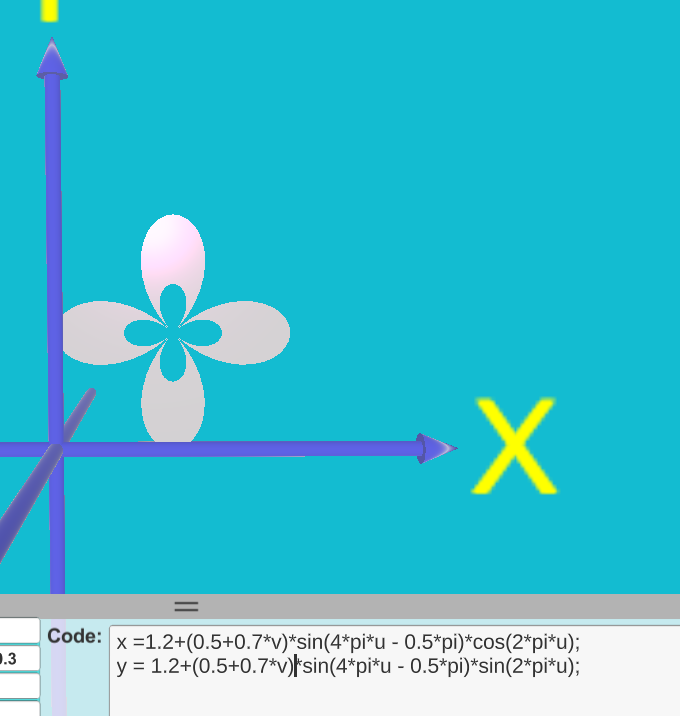
\includegraphics[width=4cm]{fig/q2ans.PNG}
        \centering
    \end{figure}
\end{homeworkProblem}

\pagebreak
\begin{homeworkProblem}
    Define parametrically with functions \(x (u, v, w)\), \(y (u, v, w)\), \(z (u, v, w)\),
    \(u, v, w \in [0, 1]\) the solid object displayed in Figure Q3. The object is created by
    rotational sweeping counterclockwise by \(5\pi/4\) about axis Y of the sinusoidal
    curve followed by translational sweeping by +1.5 units parallel to axis Y.
    \begin{figure}[H]
        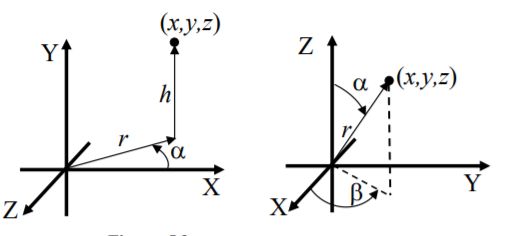
\includegraphics[width=4cm]{fig/q3.PNG}
        \centering
    \end{figure}

    \textbf{Solution}\\
    1. Define the sine wave:\\
    Amplitude: 0.2\\
    Periods: 1.5\\
    x: from 0.5 to 1.75\\
    y offset: -0.5\\
    \(x(u) = 0.5 + 1.25 u\)\\
    \(y(u) = 0.2sin(3\pi u) - 0.5\)\\\\
    2. Perform counterclockwise sweeping:\\
    \(x(u,v) = (0.5 + 1.25 u)sin(\frac{5\pi}{4}v - \frac{5\pi}{4})\)\\
    \(y(u,v) = 0.2sin(3\pi u) - 0.5\)\\
    \(z(u,v) = (0.5 + 1.25 u)cos(\frac{5\pi}{4}v - \frac{5\pi}{4})\)\\\\
    3. Perform translational sweeping:\\
    \(x(u,v,w) = (0.5 + 1.25 u)sin(\frac{5\pi}{4}v - \frac{5\pi}{4})\)\\
    \(y(u,v,w) = 0.2sin(3\pi u) - 0.5 + 1.5w\)\\
    \(z(u,v,w) = (0.5 + 1.25 u)cos(\frac{5\pi}{4}v - \frac{5\pi}{4})\)\\
    \(u,v,w \in [0,1]\)
    \begin{figure}[H]
        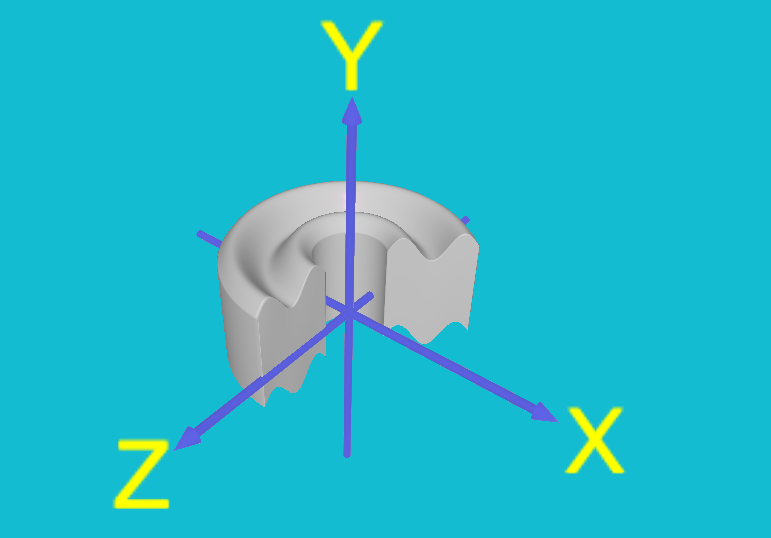
\includegraphics[width=5cm]{fig/q3ans.PNG}
        \centering
    \end{figure}


\end{homeworkProblem}

\pagebreak
\begin{homeworkProblem}
    The solid object displayed in Figure Q4 (front and back views) is constructed
    from a 3-sided pyramid with height 1 and a cylinder which has the height 2, the
    outer radius 0.5, and the inner radius 0.25. 
    \begin{enumerate}
        \item Define the pyramid and the cylinder by functions \(f(x,y,z)\geq0\)
        \item Based on the definition obtained in part 1, define the solid object.
    \end{enumerate}
    \begin{figure}[H]
        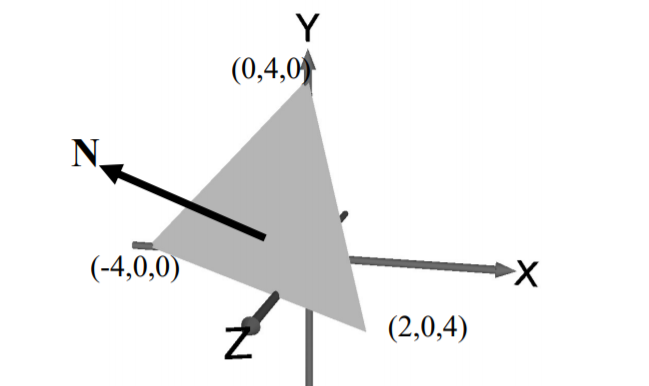
\includegraphics[width=10cm]{fig/q4.PNG}
        \centering
    \end{figure}

    \textbf{Solution}\\
    Part 1:
    Pyramid Components: 
    \begin{itemize}
        \item \(-(\frac{x}{2}+\frac{y}{1}+\frac{z}{2}-1)\geq0\), or \(\mathbf{a(x,y,z) = -x - 2y - z +2\geq0}\)
        \item \(-(\frac{x}{-2}+\frac{y}{1}+\frac{z}{2}-1)\geq0\), or \(\mathbf{b(x,y,z) = -2y + x - z + 2\geq0}\)
        \item \(y \leq 1\), or \(\mathbf{c(x,y,z) = 1 - y \geq 0}\)
        \item \(\mathbf{d(x,y,z) = y \geq 0}\)
        \item \(\mathbf{e(x,y,z) = z \geq 0}\)
    \end{itemize}
    \(\therefore \mathbf{f_{pyramid}(x,y,z) = min(a(x,y,z),b(x,y,z),c(x,y,z),d(x,y,z),e(x,y,z))\geq0}\)
    \begin{figure}[H]
        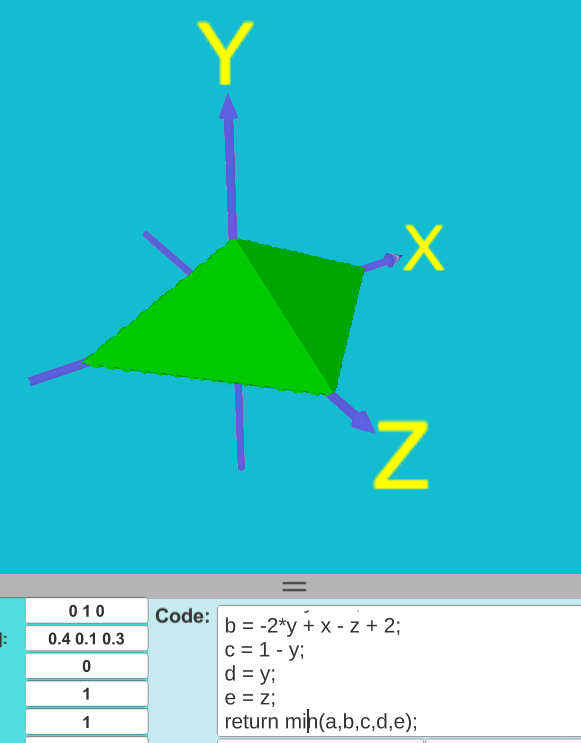
\includegraphics[width=5cm]{fig/q4pyramid.PNG}
        \centering
    \end{figure}
    \pagebreak
    Cylinder Components:\\
    Big Cylinder:
    \begin{itemize}
        \item \(\mathbf{a(x,y,z) = 0.5^2 - x^2 - z^2 \geq 0}\)
        \item \(\mathbf{b(x,y,z) = y \geq 0}\)
        \item \(\mathbf{c(x,y,z) = 2 - y \geq 0}\)        
        \item \(\mathbf{d(x,y,z) = z \geq 0}\)
    \end{itemize}
    \(\therefore \mathbf{f_{bigCyl}(x,y,z) = min(a(x,y,z),b(x,y,z),c(x,y,z),d(x,y,z))\geq0}\)

    Small Cylinder (Hollow):
    \begin{itemize}
        \item \(\mathbf{a(x,y,z) = 0.25^2 - x^2 - z^2 \geq 0}\)
        \item \(\mathbf{b(x,y,z) = y \geq 0}\)
        \item \(\mathbf{c(x,y,z) = 2 - y \geq 0}\)        
        \item \(\mathbf{d(x,y,z) = z \geq 0}\)
    \end{itemize}
    \(\therefore \mathbf{f_{smallCyl}(x,y,z) = min(a(x,y,z),b(x,y,z),c(x,y,z),d(x,y,z))\geq0}\)

    \(\therefore \mathbf{f_{cyl}(x,y,z) = min(f_{bigCyl}(x,y,z),-f_{smallCyl}(x,y,z))\geq0}\)
    \begin{figure}[H]
        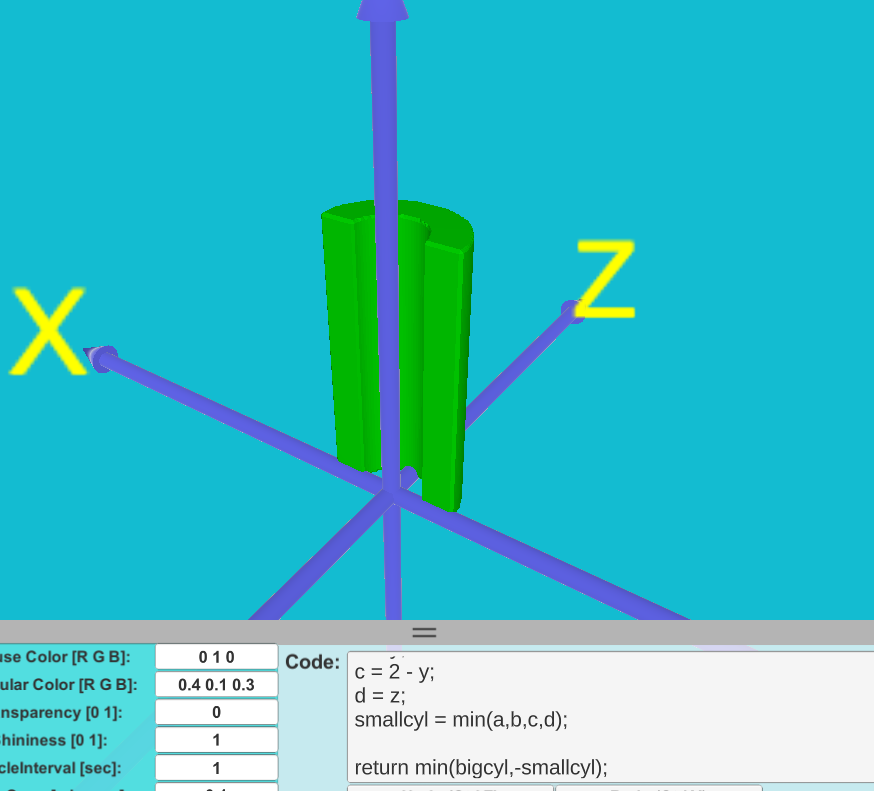
\includegraphics[width=5cm]{fig/q4cyl.PNG}
        \centering
    \end{figure}

    Part 2:\\\\
    To get the figure, union the big cylinder and pyramid, then subtract the small cylinder.

    \(\mathbf{f_{final}(x,y,z) = min(max(f_{pyramid}(x,y,z),f_{bigCyl}(x,y,z)),-f_{smallCyl}(x,y,z))\geq0}\)
    \begin{figure}[H]
        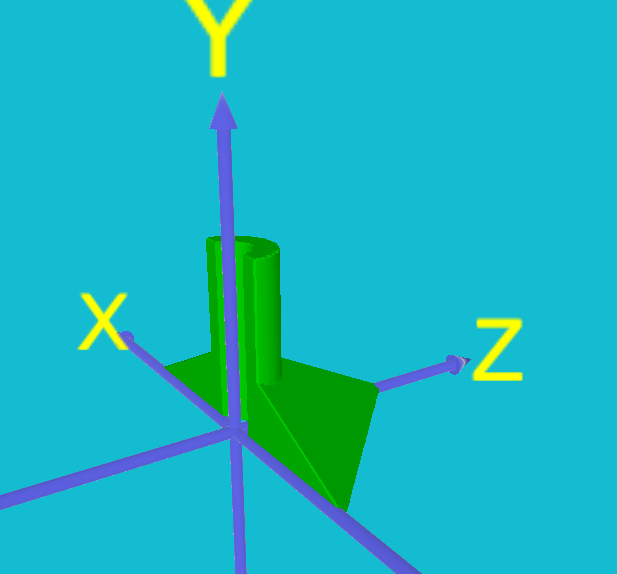
\includegraphics[width=5cm]{fig/q4final.PNG}
        \centering
    \end{figure}
\end{homeworkProblem}

\end{document}